%%%%%%%%%%%%%%%%%% ATLAS

\section{The ATLAS Experiment}
\label{sed:cern:atlas}

ATLAS (A Toroidal LHC ApparatuS)\cite{atlas:atlas}

\begin{figure}[ht]
\centering
\subfigure{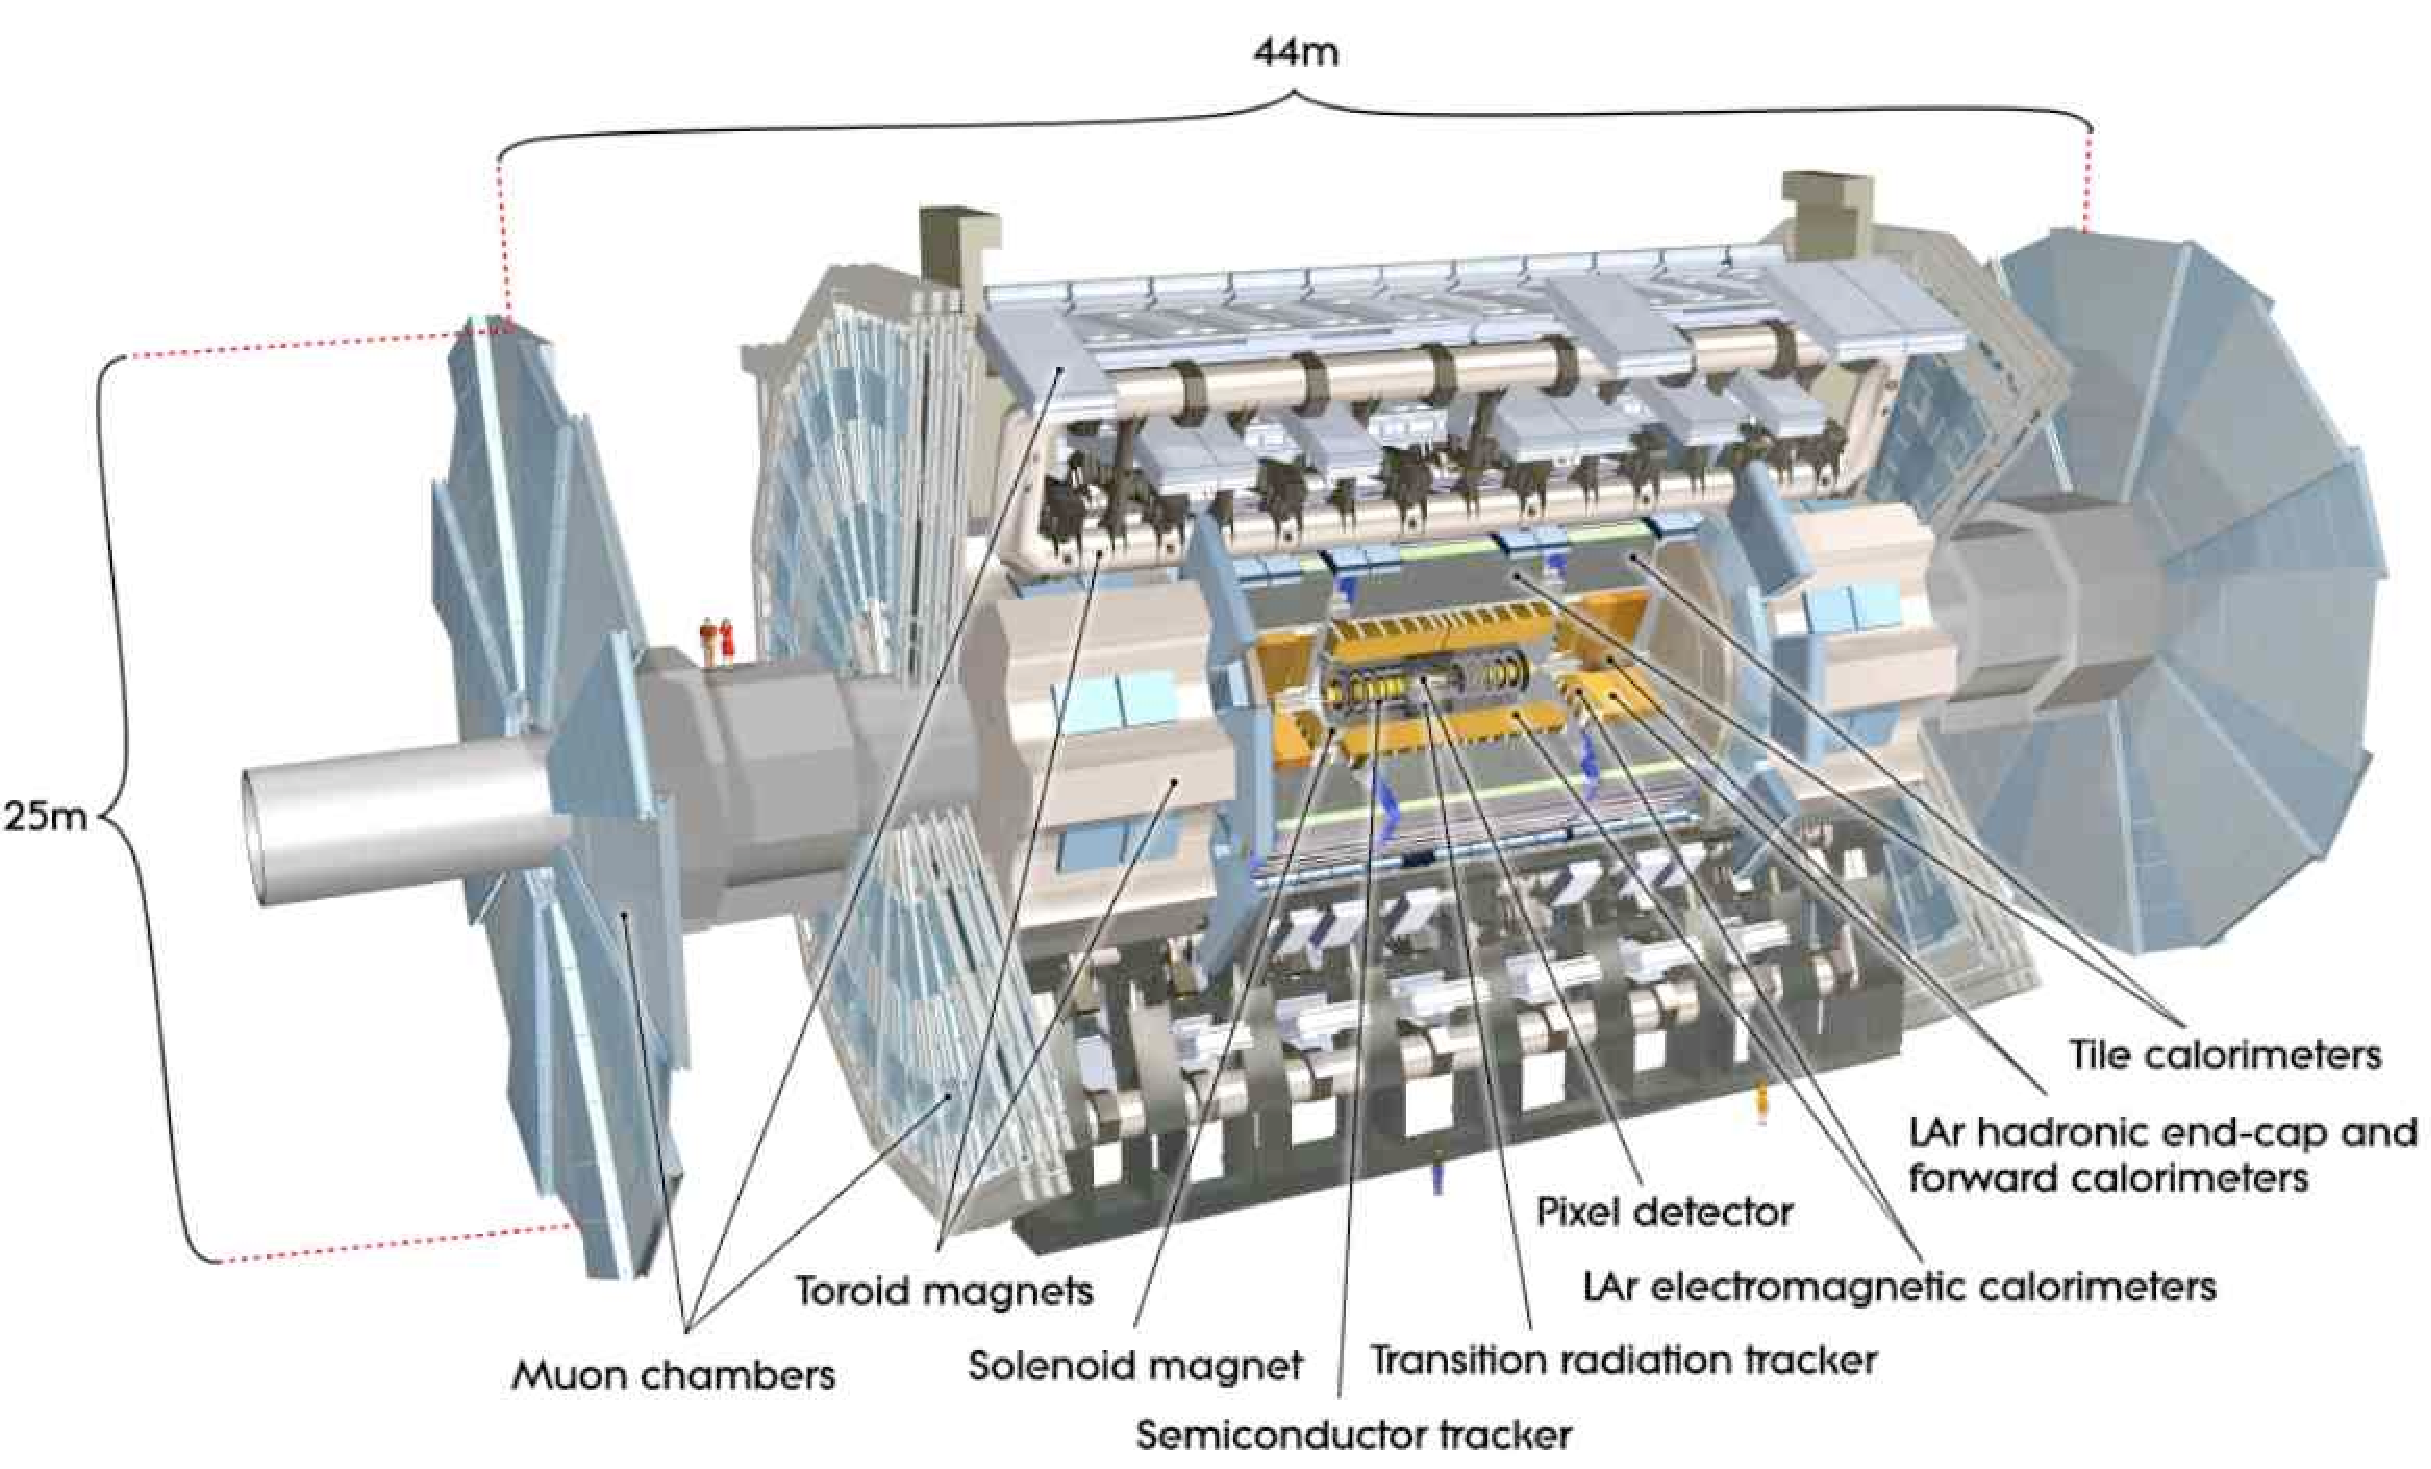
\includegraphics[width=0.85\textwidth]{figures/atlas/atlas}}
\caption{Layout of the ATLAS inner detector. Figure from Ref. \cite{atlas:atlas}}
\label{fig:atlas:atlas}
\end{figure}

\subsection{Coordinate System}

\begin{equation}
\label{eq:cern:eta}
\eta = - \ln \tan \frac{\theta}{2}
\end{equation}

\begin{equation}
\label{eq:cern:y}
y = \frac{1}{2} \ln \frac{E + p_z}{E - p_z}
\end{equation}

\begin{equation}
\label{eq:cern:pt}
p_T = \sqrt{p_x^2 + p_y^2}
\end{equation}

\begin{equation}
\label{eq:cern:pz}
p_z = p_T \,\sinh \eta
\end{equation}

\begin{equation}
\label{eq:cern:dR}
\Delta R = \sqrt{ \Delta \phi^2 + \Delta \eta^2  }
\end{equation}




\subsection{Magnet System}

\label{sec:cern:atlasmagnets}
\begin{figure}[ht]
\centering
\subfigure{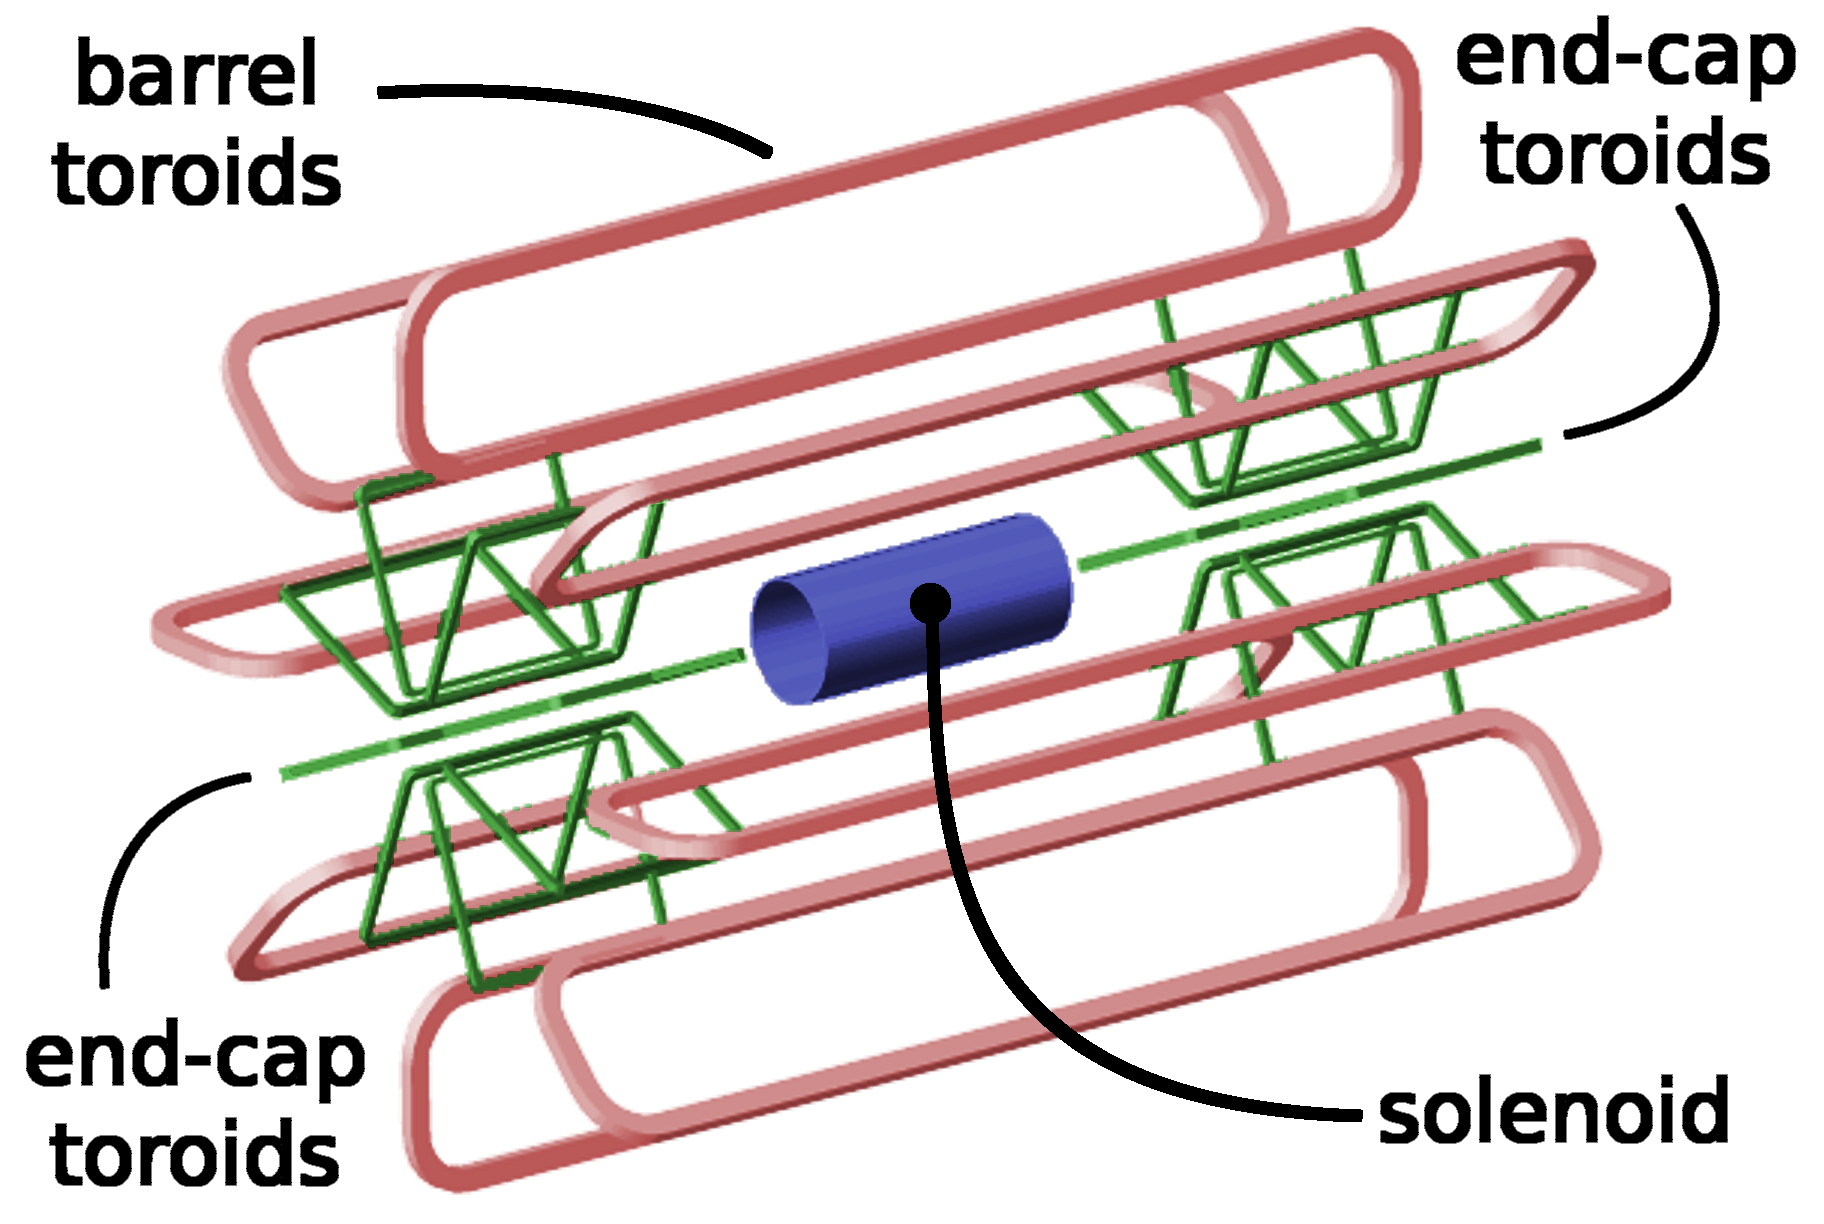
\includegraphics[width=0.35\textwidth]{figures/atlas/magnets}}
\caption{Layout of the ATLAS magnet system. Figure from Ref. \cite{Goodson}}
\label{fig:atlas:magnet}
\end{figure}



\subsubsection*{Solenoid}

\subsubsection*{Toroids}



\subsection{Inner Detector}

\begin{figure}[ht]
\centering
\subfigure{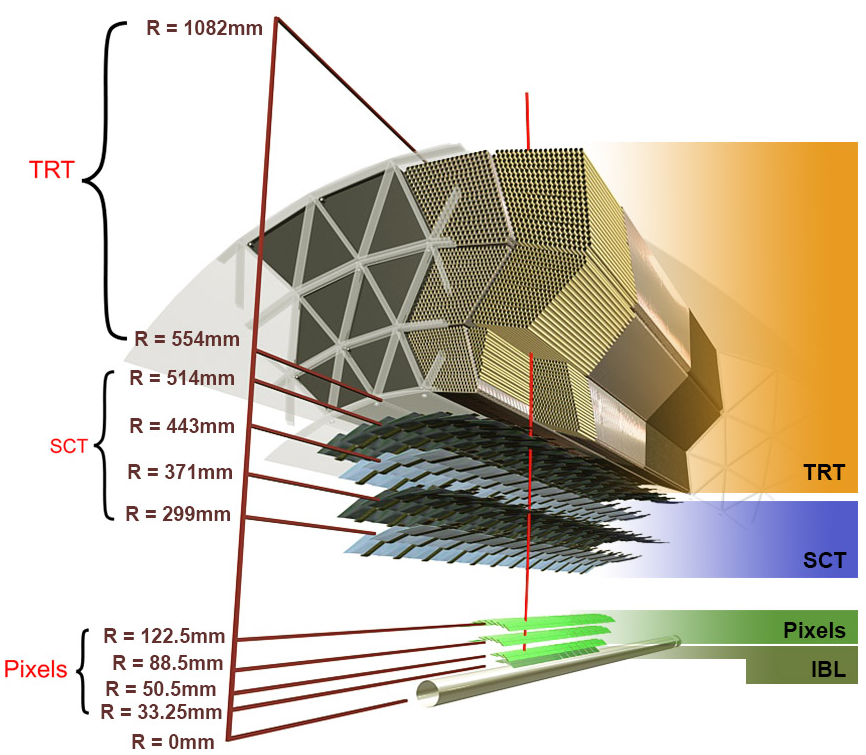
\includegraphics[width=0.65\textwidth]{figures/atlas/inner_detector}}
\caption{Layout of the ATLAS inner detector. Figure from Ref. \cite{Potamianos:2016ptf}}
\label{fig:atlas:id}
\end{figure}


\subsubsection*{Pixel Detector}


\subsubsection*{Semi-Conductor Tracker}


\subsubsection*{Transition Radiation Tracker}



\subsection{Calorimeters}

\begin{figure}[ht]
\centering
\subfigure{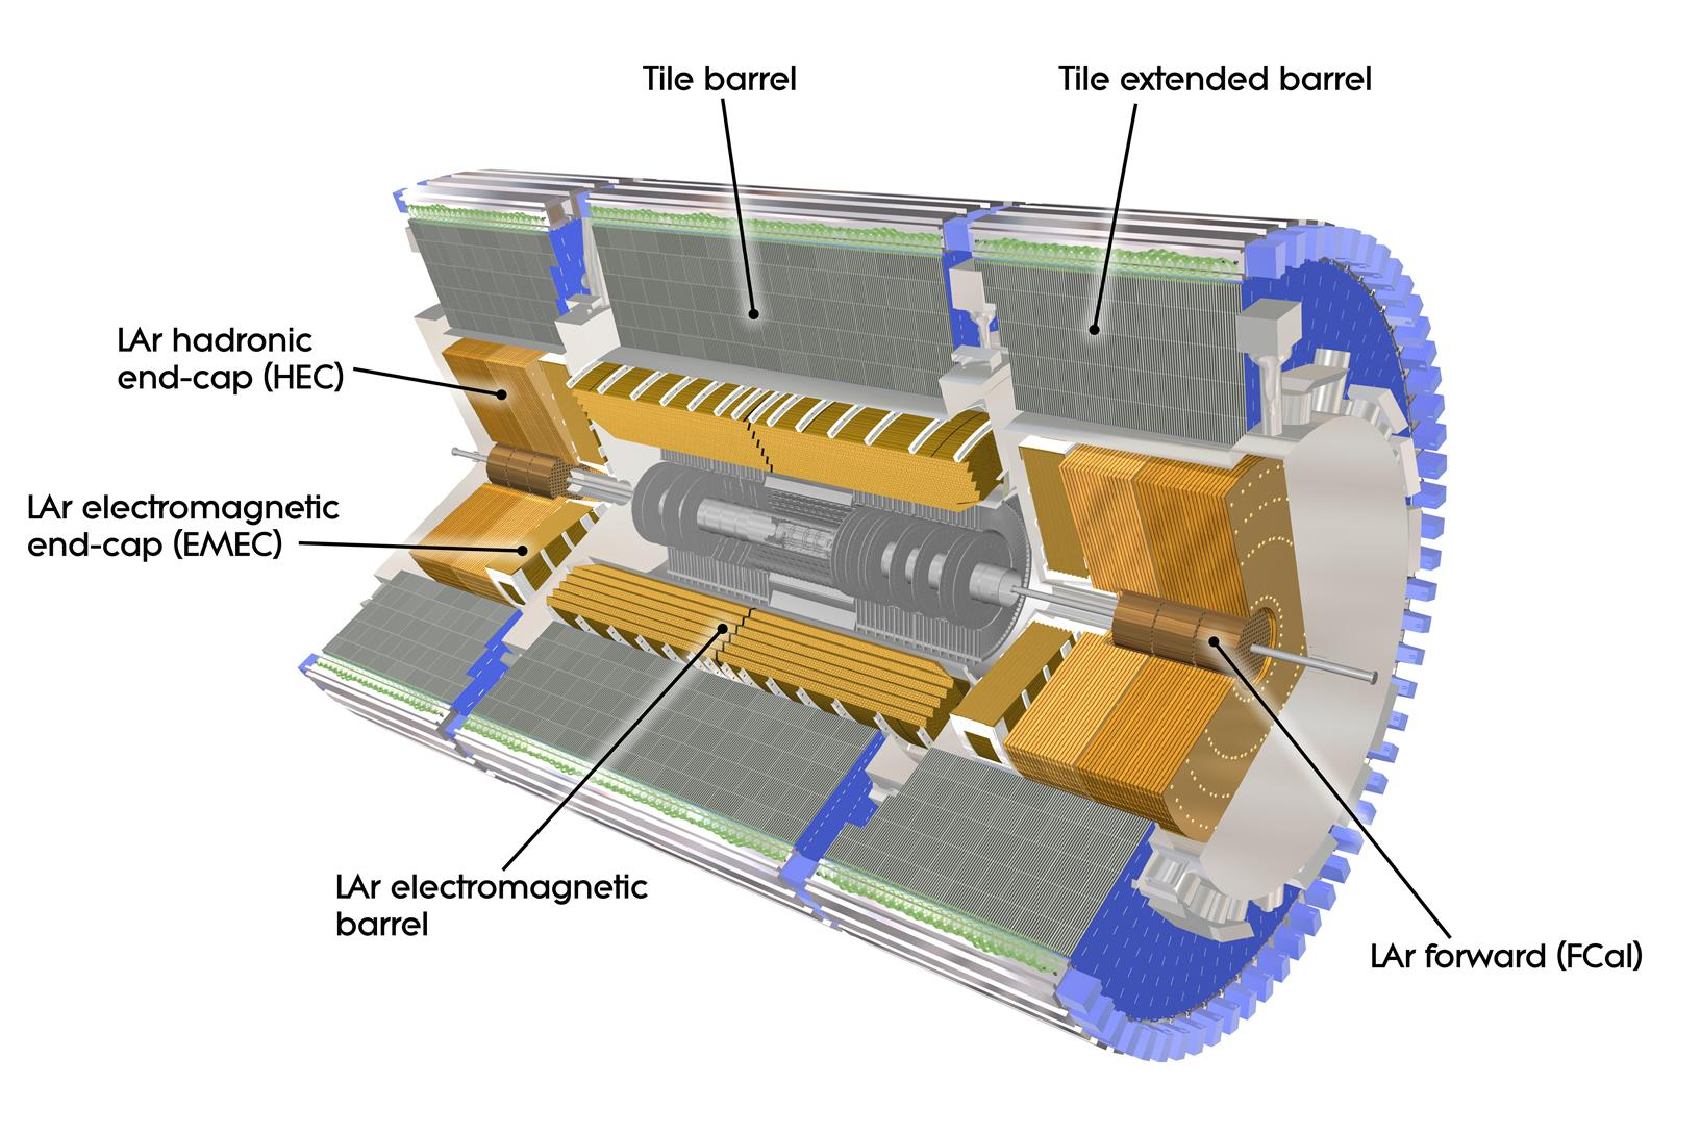
\includegraphics[width=0.75\textwidth]{figures/atlas/calorimeters}}
\caption{Layout of the ATLAS calorimeter system. Figure from Ref. \cite{atlas:atlas}}
\label{fig:atlas:calo}
\end{figure}

\subsubsection*{Electromagnetic Calorimeter}


\subsubsection*{Hadronic Calorimeter}


\subsubsection*{Forward Calorimeter}


\subsection{Muon Spectrometer}

\begin{figure}[ht]
\centering
\subfigure{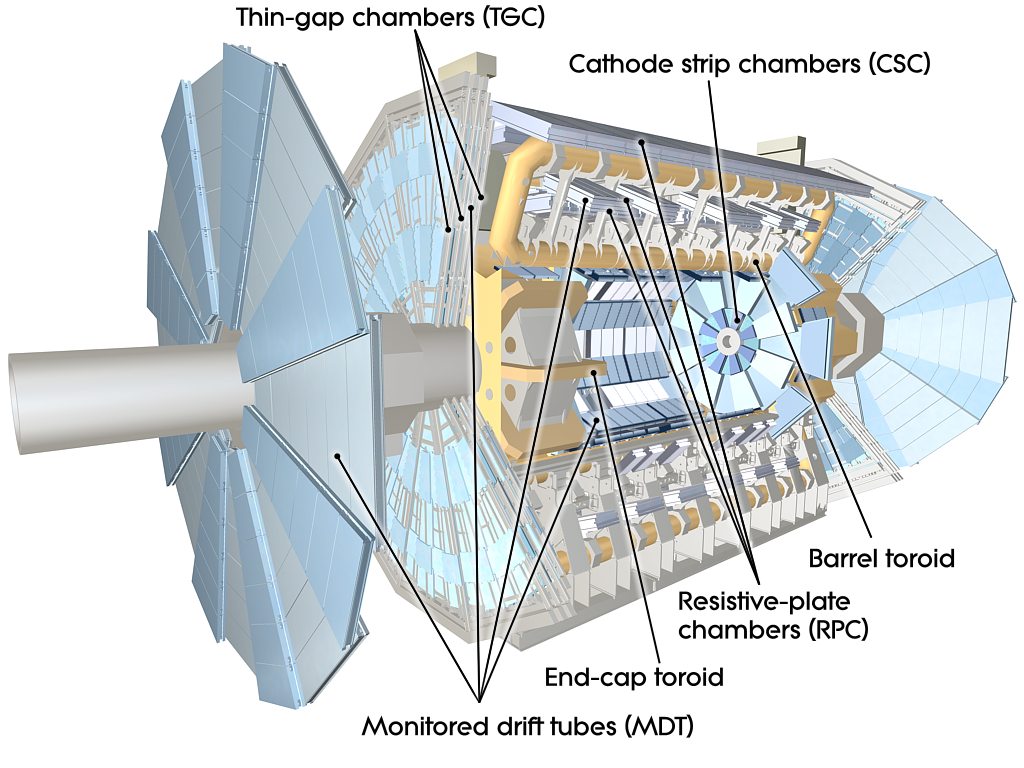
\includegraphics[width=0.65\textwidth]{figures/atlas/muon}}
\caption{Layout of the ATLAS muon system. Figure from Ref. \cite{atlas:atlas}}
\label{fig:atlas:muon}
\end{figure}

\subsection{Luminosity Detectors}

\subsection{Trigger System}
\label{sec:cern:trigger}

\subsection{ATLAS Performance Summary}


\subsection{ATLAS Physics Program}